\documentclass[conference]{IEEEtran}

\usepackage{textcomp}% for symbols
\usepackage{graphicx}
\usepackage{tabularx}
\usepackage{cite}
%\newtheorem{defi}{Definition}

\begin{document}

\title{Short Course of \LaTeX}

\author{
\authorblockN{Tsung-Lin Tsai}\\
\authorblockA{
Graduate Institute of Communication Engineering\\
National Taiwan University\\
Taipei, R.O.C\\
R95942101@ntu.edu.tw}
}

\maketitle

%\begin{abstract}
%In this report, we will first discuss the technologies of video
streaming in other papers. Then our efforts provide the conclusion
of the papers to find out their defects, and we can know the
related future works for us to follow the direction of this issue.
%\end{abstract}

\section{Introduction}
\PARstart{T}he wireless mesh network (WMN) is a kind of ad-hoc
networks, where nodes are willing to forward data for other nodes
and the transmission path is determined dynamically based on the 
network connectivity, with full or partial mesh topologies.

\section{Overview}

%\cite{belair}, SkyPilot\footnote{It is a company}, BearCom, and so
%on.

\subsection{Atmospheric dispersion modeling}
In order to simulate the air pollution, we find out a well known air dipersion 
model which is a partial differential equation based on the law of 
conservation of mass. The solution of this differential equation can give us 
a function coordination to calculate the mass concentration of every point in 
the space.  

%\cite{fixed} shows an example of the most known one, video
%surveillance system. $\omega$

\subsection{Scenario}
In the atmospheric dispersion model we assumed that the wind speed and direction
is already known. However, in more realize case this assumption is over ideal 
assumption. Hence, based on this model, we relax the restriction of information 
about wind and make the wind speed as a random variable with some resonable 
distribution. Then we set up the  pollutant concentration sensor which distributed
uniformly as the cellular base station. 

\subsection{Algorthm}
When the pollutant is spreading in the space, the sensor start sensing the 
pollutant concentration nearby itself, and retrainsmitting the data back to the 
cluster head. After that, server will reconstruct the pollutant distribution map 
which can point out that some certain area suffer from the pollutant seriously.
On the other hand, our wireless sensor might be restricted by the channel capacity
 


%\begin{figure}
%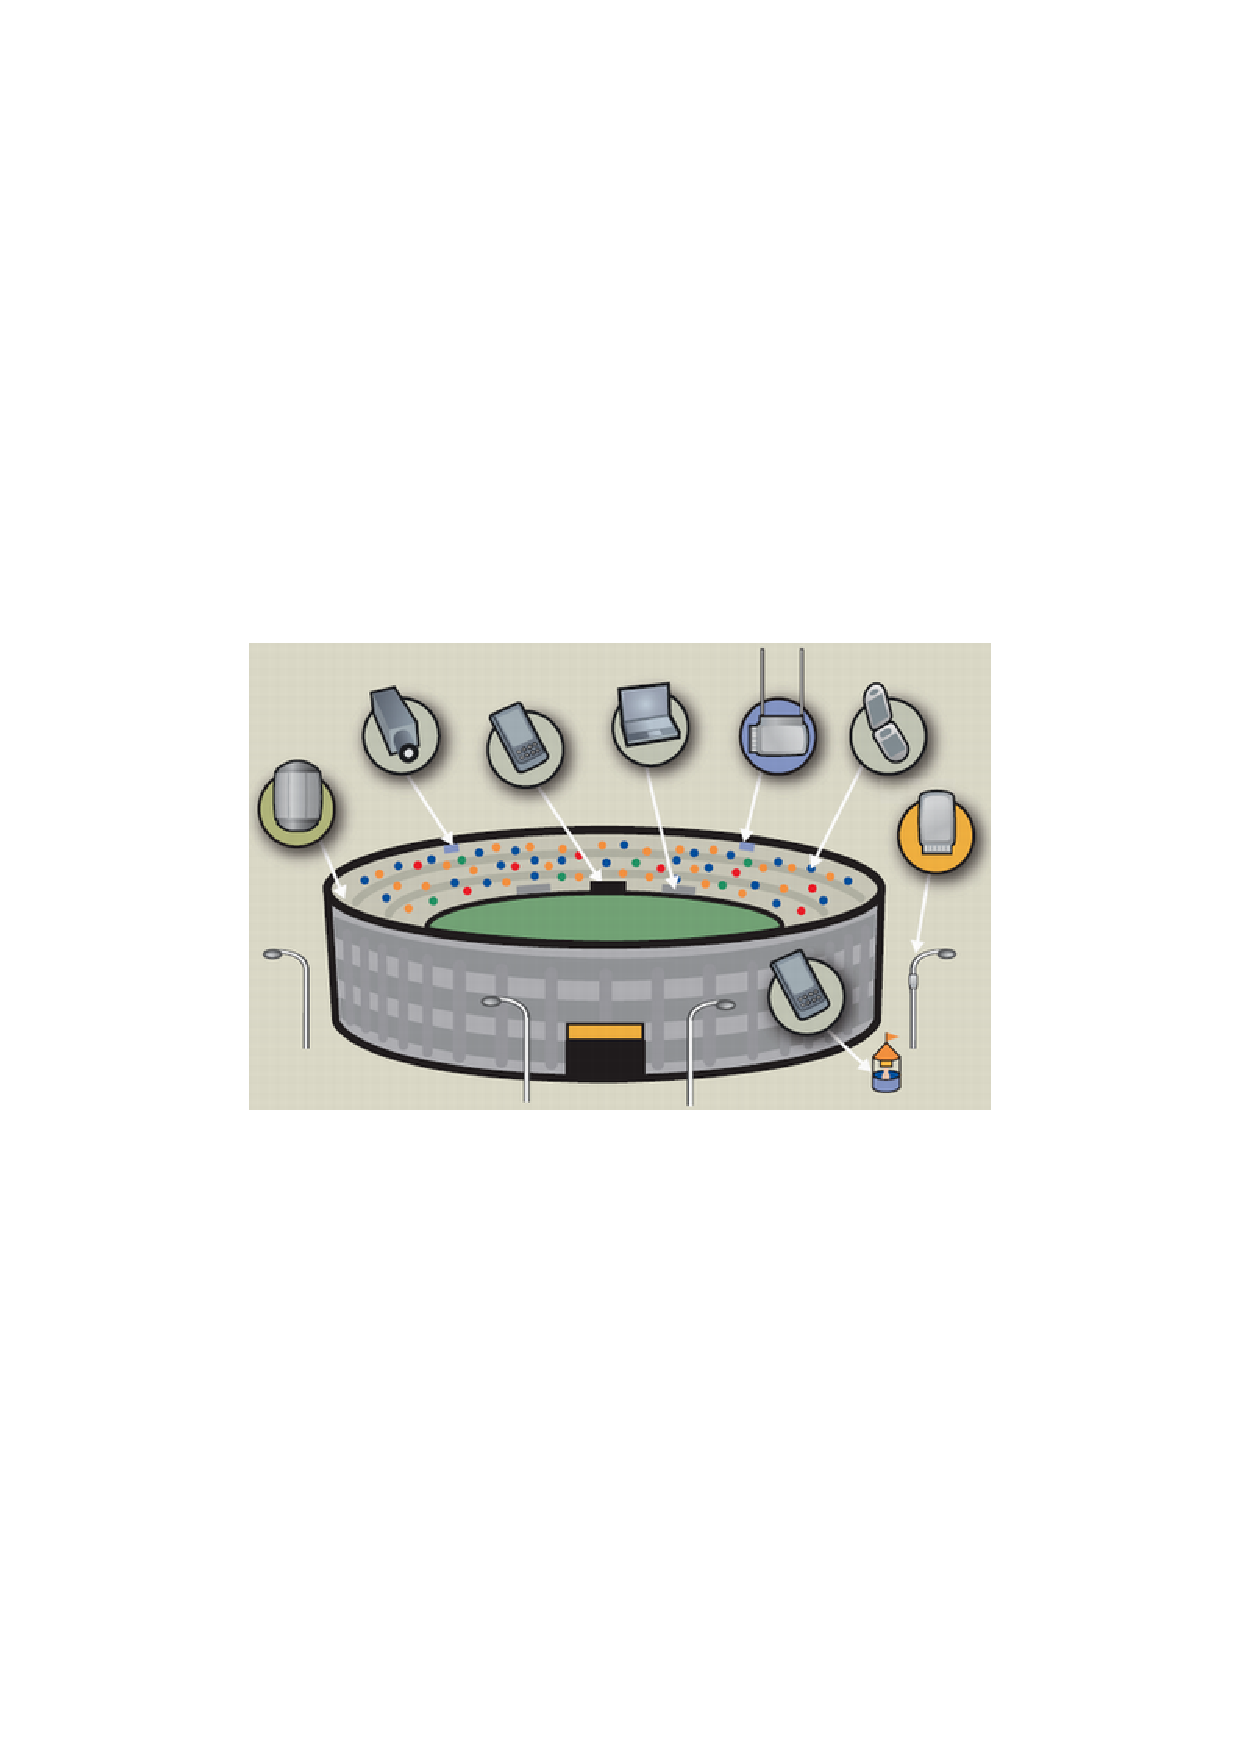
\includegraphics[scale=0.7 ,angle=0]{gym}
%\caption{A WMN video streaming topology in the gym}
%\label{gym}
%\end{figure}

%\begin{figure}
%\includegraphics[scale=0.8 ,angle=0,bb=140 300 470 520, clip]{video}
%\caption{The surveillance system over WMNs} \label{video}
%\end{figure}

==========================
\begin{itemize}
\item first big item 
\item second big item
\begin{itemize}
\item first small item 
\item second small item
\end{itemize}
\item third big item
\end {itemize}

==========================

\begin{enumerate}
\item first big item 
\item second big item
\begin{enumerate}
\item first small item 
\item second small item
\end{enumerate}
\item third big item
\end {enumerate}

==========================

\begin{description}
\item[Bill] first big item 
\item[Mary] second big item
\begin{description}
\item[Soft] first small item 
\item[Hard] second small item
\end{description}
\item[Jack] third big item
\end {description}

==========================
\begin{table}
\caption{Characteristics}
\begin{center}
\begin{tabular}{lll}
\hline
 & \multicolumn{2}{c}{\bf Specific Heats} \\
\cline{2-3}
 & $c$ (J/kg$\cdot$K) & $C$ (J/mol$\cdot$K) \\
\hline
Aluminum     & 900  & 24.3 \\
Copper       & 385  & 24.4 \\
Gold         & 130  & 25.6 \\
Steel/Iron   & 450  & 25.0 \\
Lead         & 130  & 26.8 \\
Mercury      & 140  & 28.0 \\
Water        & 4190 & 75.4 \\
Ice ($-$10 \textcelsius) & 2100 & 38 \\
\hline
\end{tabular}
\end{center}
\label{TABLE}
\end{table}

\begin{figure}
\begin{center}
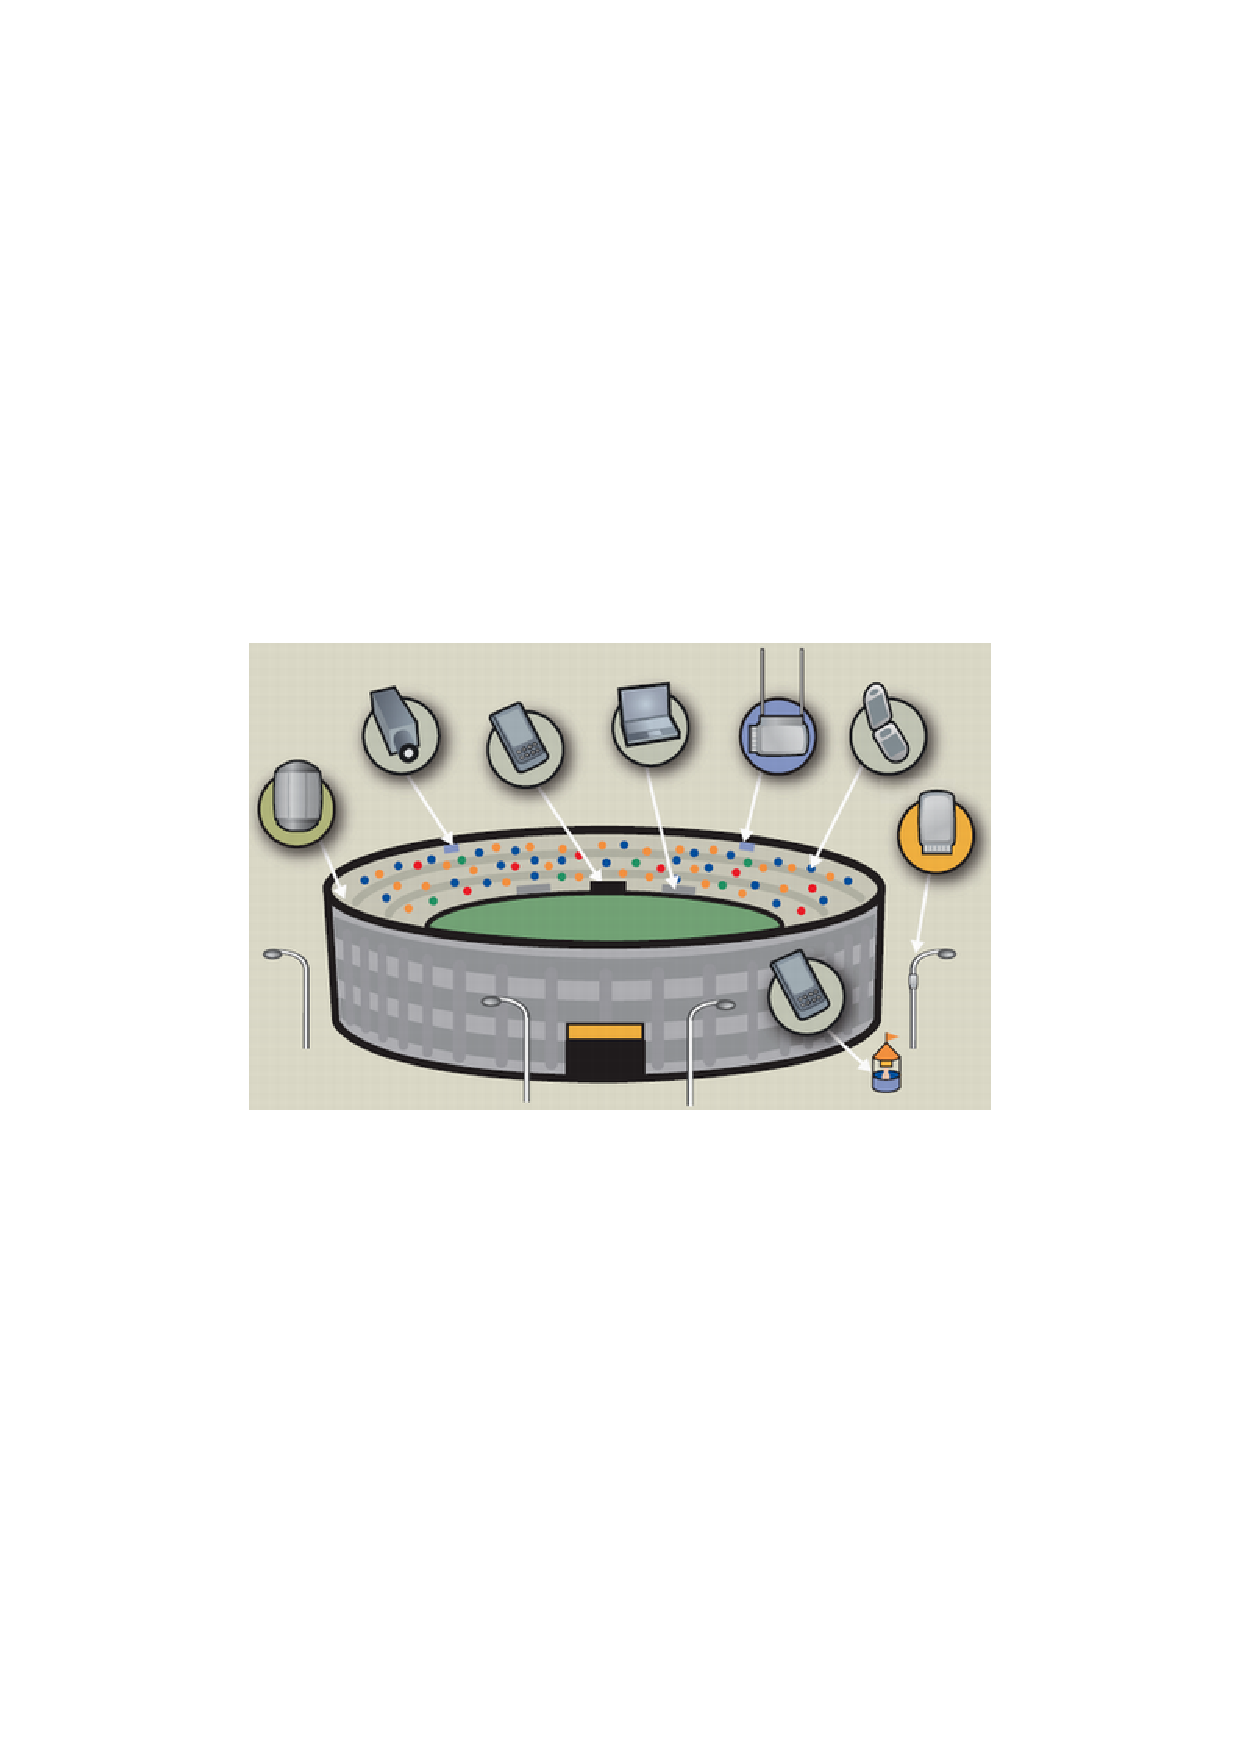
\includegraphics[width=0.8\columnwidth ,angle=0]{gym}
\caption{A WMN video streaming topology in the gym}
\label{gym}
\end{center}
\end{figure}

\section{Model of Video Streaming}
\subsection{Video Distortion Model}
In \cite{distortion}, it introduces this video distortion model.
For this concurrent video streaming application, video packets are
transmitted over the wireless mesh network and need to meet their
playout deadline. Then the decoded video distortion, $D_{dec}$, is
given by:

\begin{equation} D^{dec} = D_{enc} + D_{loss} \end{equation}
\begin{equation} D_{enc} = D_{0} + \theta/(R-R_{0}) \end{equation}
\begin{equation} D_{loss} = k(P_{v} + [1-P_{v}](1-P(T_v>\delta_v))) \end{equation}

. In \cite{distortion}, the parameters of the model are
$D_0=0.49$, $\theta=1222$, $R_0=10.39kbps$, $k=185$.

\subsection{Network Model}
Before we introduce the network model, we should define some
parameters first \cite{belair,GA,fixed}. Consider a WMN with N
nodes distributed on a plane with $c_{ij}$ as the distance between
two nodes $i$ and $j$. Each wireless mesh node is equipped with a
radio having transmission range $r_i$ and interference range
$r'_i$. Hence, we can model such a WMN by a directed graph
$\mathbf{G=G(N,L)}$, where $\mathbf{N}$ represents the set of
nodes in the WMN, and $\mathbf{L}$ represents the set of wireless
directed links between nodes. A direct link $\lbrace ij \rbrace$
exists from node $i$ to node $j$ if $c_{ij} \le r_{i}$ and $i \ne
j$. We characterize link $\lbrace ij \rbrace \in \mathbf{L}$
using:

Besides, we let the path of video clip $v$ be $L_v$, which
includes a set of link $\lbrace ij \rbrace$. For each link
$\lbrace ij \rbrace$ we define an index variable:

\begin{equation}
X_{ij}^v = \left\{\begin{array}{ll}
  1,  & \lbrace ij \rbrace \in L_v\\
  0,  & \lbrace ij \rbrace \notin L_v
\end{array} \right. \forall \lbrace ij \rbrace \in \mathbf{L}, \forall v \in
\mathbf{V}
\end{equation}

\subsubsection{Packet loss rate and delay}
Assume that the bit error rate (BER) on link $\lbrace ij \rbrace$
is $e_{ij}$, and S is the average packet size. Then the end-to-end
packet loss rate associated with path $L_v$ can be defined as:
\begin{equation} P_v = 1 -  \prod_{{\lbrace ij
\rbrace \in \mathbf{L}}} (1- X ^{v}_{ij}), \forall v \in
\mathbf{V}
\end{equation}

$P_{ij} = 1-(1-e_{ij})^S$ is the packet loss on link $\lbrace ij
\rbrace$.

\subsubsection{Interference model}
To model the delay, we assume the delay $t_{ij}$ on link $\lbrace
ij \rbrace$ is an exponential distribution with the probability
density function $f_{t_{ij}}(x) \sim \lambda e^{-\lambda_{ij}x}$,
$\forall \lbrace ij \rbrace \in \mathbf{L}$. As a result, the
end-to-end delay for path $L_v$ can be derived as:

When the number of hops along $L_v$ is not large enough, we use
the moment generating function, $G_{T_v(s)}$, to find the
probability that the packet streamed over path $L_v$ has delivery
delay longer than $\delta_v$. Then we can get this probability,
$P(T_v>\delta_v)$, when the number of hops is small as
\cite{error}:

\begin{eqnarray}
P(T_v>\delta_v)&=&\int_{\delta_v}^{\infty} \, f_{T_v}(x)\, dx \nonumber\\
               &=&\sum_{\lbrace ij \rbrace \in L_v} \lbrace
(\lambda_{ij}-X_{ij}^vs)G_{T_v(s)}\rbrace \mid_{s=\lambda_{ij}} \nonumber\\
\end{eqnarray}

\subsubsection{Aggregated traffic}
In this part, we want to model the total traffic on the link
$\lbrace ij \rbrace$. And we define $L_v^i$ as the sub-path which
includes all the links along the path $L_v$ up to the link
$\lbrace ij \rbrace$. Therefore, we can derived the total traffic
on link $\lbrace ij \rbrace$, $\rho_{ij}$, as:

\begin{equation} \rho_{ij} = \sum_{v \in \mathbf{V}} \prod_{{\lbrace
kn \rbrace \in L_v^i}} \lbrace(1- P_{kn})X ^{v}_{kn}\rbrace \times
R_v , \forall \lbrace ij \rbrace \in \mathbf{L} \end{equation}

%\subsubsection{Interference model}
\subsection{Route selection} Moreover, the aggregate traffic
on each link $\lbrace ij \rbrace$ should be guaranteed that it can
not exceed its available bandwidth $R_{ij}$. Hence, the problem of
routing loop also should be prevented. After concluding the above
constraints, we can formulate the optimal route selection problem
as: given a WMN $\mathbf{G(N,L)}$ and a set of video clips, for
$\mathbf{V}$ streaming requests, find a set of paths so that the
aggregate distortion of $\mathbf{V}$ concurrent video sessions is
minimized. And this route selection problem can be mathematic
formulated as:

\begin{itemize}
\item Minimize:
\begin{equation}
\sum_{v \in \mathbf{V)}} D_v
\end{equation}
\item Subject to:

\begin{equation}
\rho_{ij} \le R_{ij}, \forall \lbrace ij \rbrace \in \mathbf{L}
\end{equation}

\begin{eqnarray}
\sum_{j:\lbrace ij \rbrace \in L_v} X_{ij}^v
\left\{\begin{array}{ll}
  =0,    & i: i \in L_v, L_v^i = \Phi\\
  \le1,  & otherwise
\end{array} \right.,\nonumber\\
\forall i \in \mathbf{N}, \forall v \in \mathbf{V}
\end{eqnarray}

\end{itemize}

where $D_v$ is the average distortion of received video clip $v$
at the receive node $\gamma_v$. (10) is the rate constraint to
satisfy. (11), (12), and (13) guarantee each path $L_v$ provides a
loop-free connection.
\section{Conclusion}
%\label{con}
In this report, we first conclude the applications of video
streaming over WMNs.


% Introduction
	% 學長有一個演算法,找尋適合的scenario來符合需求
	% 為了救災之類的
% Overview
	% Model: 找到一個被廣泛使用的空氣汙染model
	% Scenario: 為什麼要讓風速和風向為random variable
	% Algorithm: 介紹一下他的Complexity,他是一個解最佳化問題的方法
% Model
% Scenario
% Algorithm
% Simulation
% Result
% Reference

\bibliographystyle{IEEEtran}
\bibliography{bio} % Reference

\end{document}
